%% Created by Maple 2016.0, Windows 7
%% Source Worksheet: ������� ������ � ���������� piecewice.mw
%% Generated: Thu Oct 10 14:19:27 EEST 2024
\documentclass{article}
\usepackage{maplestd2e}
\def\emptyline{\vspace{12pt}}
\begin{document}
\pagestyle{empty}
\DefineParaStyle{Maple Bullet Item}
\DefineParaStyle{Maple Heading 1}
\DefineParaStyle{Maple Warning}
\DefineParaStyle{Maple Heading 4}
\DefineParaStyle{Maple Heading 2}
\DefineParaStyle{Maple Heading 3}
\DefineParaStyle{Maple Dash Item}
\DefineParaStyle{Maple Error}
\DefineParaStyle{Maple Title}
\DefineParaStyle{Maple Text Output}
\DefineParaStyle{Maple Normal}
\DefineCharStyle{Maple 2D Output}
\DefineCharStyle{Maple 2D Input}
\DefineCharStyle{Maple Maple Input}
\DefineCharStyle{Maple 2D Math}
\DefineCharStyle{Maple Hyperlink}
\begin{Maple Normal}{
\begin{Maple Normal}{
}\end{Maple Normal}
}\end{Maple Normal}
\begin{Maple Normal}{
\begin{Maple Normal}{
Применима ли теорема Гаусса к потенциалу Лиенара Вихерта}\end{Maple Normal}

}\end{Maple Normal}

\begin{Maple Normal}{
\begin{Maple Normal}{
}\end{Maple Normal}
}\end{Maple Normal}
\begin{Maple Normal}{
\begin{Maple Normal}{
Проверим прямым вычислением применимость теоремы Гаусса в интегральном виде к потенциалу ЛВ. Для этого вычислим интеграл нормальной компоненты электрического поля в сферической системе координат.}\end{Maple Normal}

\begin{Maple Normal}{
Проверим прямым вычислением применимость теоремы Гаусса в интегральном виде к потенциалу ЛВ. Для этого вычислим интеграл нормальной компоненты электрического поля в сферической системе координат.}\end{Maple Normal}

}\end{Maple Normal}

\begin{Maple Normal}{
\begin{Maple Normal}{
}\end{Maple Normal}
}\end{Maple Normal}
\begin{Maple Normal}{
\begin{Maple Normal}{
\mapleinline{inert}{2d}{restart; -1; clear; -1}{\[\displaystyle \]}
}\end{Maple Normal}
}\end{Maple Normal}
\begin{Maple Normal}{
\begin{Maple Normal}{
}\end{Maple Normal}
}\end{Maple Normal}
\begin{Maple Normal}{
\begin{Maple Normal}{
Начало отсчёта запаздывающего времени\mapleinline{inert}{2d}{tau}{$\displaystyle \tau$}
}\end{Maple Normal}

}\end{Maple Normal}

\begin{Maple Normal}{
\begin{Maple Normal}{
\mapleinline{inert}{2d}{Tau__0 := 0; -1}{\[\displaystyle \]}
}\end{Maple Normal}
}\end{Maple Normal}
\begin{Maple Normal}{
\begin{Maple Normal}{
Величина ускорения заряда}\end{Maple Normal}

}\end{Maple Normal}

\begin{Maple Normal}{
\begin{Maple Normal}{
\mapleinline{inert}{2d}{A := .1; -1}{\[\displaystyle \]}
}\end{Maple Normal}
}\end{Maple Normal}
\begin{Maple Normal}{
\begin{Maple Normal}{
}\end{Maple Normal}
}\end{Maple Normal}
\begin{Maple Normal}{
\begin{Maple Normal}{
Начальная скорость заряда в запаздывающий момент времени \mapleinline{inert}{2d}{Tau__0}{$\displaystyle {\it Tau}_{0}$}
}\end{Maple Normal}

}\end{Maple Normal}

\begin{Maple Normal}{
\begin{Maple Normal}{
\mapleinline{inert}{2d}{V := 0; -1}{\[\displaystyle \]}
}\end{Maple Normal}
}\end{Maple Normal}
\begin{Maple Normal}{
\begin{Maple Normal}{
}\end{Maple Normal}
}\end{Maple Normal}
\begin{Maple Normal}{
\begin{Maple Normal}{
Начальная координата заряда в запаздывающий момент времени \mapleinline{inert}{2d}{Tau__0}{$\displaystyle {\it Tau}_{0}$}
}\end{Maple Normal}

}\end{Maple Normal}

\begin{Maple Normal}{
\begin{Maple Normal}{
\mapleinline{inert}{2d}{Z := 0; -1}{\[\displaystyle \]}
}\end{Maple Normal}
}\end{Maple Normal}
\begin{Maple Normal}{
\begin{Maple Normal}{
}\end{Maple Normal}
}\end{Maple Normal}
\begin{Maple Normal}{
\begin{Maple Normal}{
Радиус сферической поверхности интегрирования}\end{Maple Normal}

}\end{Maple Normal}

\begin{Maple Normal}{
\begin{Maple Normal}{
\mapleinline{inert}{2d}{R := 1; -1}{\[\displaystyle \]}
}\end{Maple Normal}
}\end{Maple Normal}
\begin{Maple Normal}{
\begin{Maple Normal}{
}\end{Maple Normal}
}\end{Maple Normal}
\begin{Maple Normal}{
\begin{Maple Normal}{
Зададим уравнение движение заряда в зависимости от запаздывающего момента tau}\end{Maple Normal}

}\end{Maple Normal}

\begin{Maple Normal}{
\begin{Maple Normal}{
Пусть заряд изначально покоившийся в момент времени \mapleinline{inert}{2d}{tau__0}{$\displaystyle \tau_{0}$}
приобретает ускорение в направлении оси z}\end{Maple Normal}

}\end{Maple Normal}

\begin{Maple Normal}{
\begin{Maple Normal}{
Таким образом уравнение движение заряда можно выразить в виде кусочно-непрерывной функции}\end{Maple Normal}

}\end{Maple Normal}

\begin{Maple Normal}{
\begin{Maple Normal}{
\mapleinline{inert}{2d}{a__q := proc (a__0, tau, tau__0) options operator, arrow; piecewise(tau__0 < tau, a__0, 0) end proc; -1}{\[\displaystyle \]}
}\end{Maple Normal}
}\end{Maple Normal}
\begin{Maple Normal}{
\begin{Maple Normal}{
\mapleinline{inert}{2d}{a__q(a__0, tau, tau__0)}{\[\displaystyle a_{q} \left( a_{0},\tau,\tau_{0} \right) \]}
}\end{Maple Normal}
}\end{Maple Normal}
\begin{maplegroup}
\begin{Maple Normal}{
\mapleinline{inert}{2d}{a__q(a__0, tau, tau__0)}{\[\displaystyle a_{q} \left( a_{0},\tau,\tau_{0} \right) \]}
}\end{Maple Normal}
\mapleresult
\begin{maplelatex}
\mapleinline{inert}{2d}{piecewise(tau__0 < tau, a__0, 0)}{\[\displaystyle \cases{a_{0}&$\tau_{0}<\tau$\cr 0&otherwise\cr}\]}
\end{maplelatex}
\end{maplegroup}
\begin{Maple Normal}{
\begin{Maple Normal}{
}\end{Maple Normal}
}\end{Maple Normal}
\begin{Maple Normal}{
\begin{Maple Normal}{
\mapleinline{inert}{2d}{z__q := proc (z__0, v__0, a__0, tau, tau__0) options operator, arrow; piecewise(tau__0 < tau, z__0+v__0*(tau-tau__0)+(1/2)*a__0*(tau-tau__0)^2, z__0+v__0*(tau-tau__0)) end proc; -1}{\[\displaystyle \]}
}\end{Maple Normal}
}\end{Maple Normal}
\begin{Maple Normal}{
\begin{Maple Normal}{
\mapleinline{inert}{2d}{z__q(z__0, v__0, a__0, tau, tau__0)}{\[\displaystyle z_{q} \left( z_{0},v_{0},a_{0},\tau,\tau_{0} \right) \]}
}\end{Maple Normal}
}\end{Maple Normal}
\begin{maplegroup}
\begin{Maple Normal}{
\mapleinline{inert}{2d}{z__q(z__0, v__0, a__0, tau, tau__0)}{\[\displaystyle z_{q} \left( z_{0},v_{0},a_{0},\tau,\tau_{0} \right) \]}
}\end{Maple Normal}
\mapleresult
\begin{maplelatex}
\mapleinline{inert}{2d}{piecewise(tau__0 < tau, z__0+v__0*(tau-tau__0)+(1/2)*a__0*(tau-tau__0)^2, z__0+v__0*(tau-tau__0))}{\[\displaystyle \cases{z_{0}+v_{0}\, \left( \tau-\tau_{0} \right) +1/2\,a_{0}\, \left( \tau-\tau_{0} \right) ^{2}&$\tau_{0}<\tau$\cr z_{0}+v_{0}\, \left( \tau-\tau_{0} \right) &otherwise\cr}\]}
\end{maplelatex}
\end{maplegroup}
\begin{Maple Normal}{
\begin{Maple Normal}{
\mapleinline{inert}{2d}{v__q := proc (v__0, a__0, tau, tau__0) options operator, arrow; piecewise(tau__0 < tau, v__0+a__0*(tau-tau__0), v__0) end proc; -1}{\[\displaystyle \]}
}\end{Maple Normal}
}\end{Maple Normal}
\begin{Maple Normal}{
\begin{Maple Normal}{
\mapleinline{inert}{2d}{v__q(v__0, a__0, tau, tau__0)}{\[\displaystyle v_{q} \left( v_{0},a_{0},\tau,\tau_{0} \right) \]}
}\end{Maple Normal}
}\end{Maple Normal}
\begin{maplegroup}
\begin{Maple Normal}{
\mapleinline{inert}{2d}{v__q(v__0, a__0, tau, tau__0)}{\[\displaystyle v_{q} \left( v_{0},a_{0},\tau,\tau_{0} \right) \]}
}\end{Maple Normal}
\mapleresult
\begin{maplelatex}
\mapleinline{inert}{2d}{piecewise(tau__0 < tau, v__0+a__0*(tau-tau__0), v__0)}{\[\displaystyle \cases{v_{0}+a_{0}\, \left( \tau-\tau_{0} \right) &$\tau_{0}<\tau$\cr v_{0}&otherwise\cr}\]}
\end{maplelatex}
\end{maplegroup}
\begin{Maple Normal}{
\begin{Maple Normal}{
Запишем уравнение для вычисления запаздывающего момента tau для вычисления электрического поля в момент времени t на сферической поверхности интегрирования радиуса\mapleinline{inert}{2d}{R__0}{$\displaystyle R_{0}$}
}\end{Maple Normal}

}\end{Maple Normal}

\begin{Maple Normal}{
\begin{Maple Normal}{
\mapleinline{inert}{2d}{Eq := proc (z__0, v__0, a__0, tau, tau__0, t, theta) options operator, arrow; c^2*(t-tau)^2 = R__0^2+z__q(z__0, v__0, a__0, tau, tau__0)^2-2*R__0*z__q(z__0, v__0, a__0, tau, tau__0)*cos(theta) end proc; -1}{$\displaystyle $}
\mapleinline{inert}{2d}{}{$\displaystyle $}
\mapleinline{inert}{2d}{}{$\displaystyle $}
}\end{Maple Normal}
}\end{Maple Normal}
\begin{Maple Normal}{
\begin{Maple Normal}{
Подставляем в это уравнение заданные числовые значения}\end{Maple Normal}

}\end{Maple Normal}

\begin{Maple Normal}{
\begin{Maple Normal}{
\mapleinline{inert}{2d}{Eqs := proc (tau, t, theta) options operator, arrow; subs(z__0 = Z, v__0 = V, a__0 = A, c = 1, R__0 = R, tau__0 = Tau__0, Eq(z__0, v__0, a__0, tau, tau__0, t, theta)) end proc; -1}{\[\displaystyle \]}
}\end{Maple Normal}
}\end{Maple Normal}
\begin{Maple Normal}{
\begin{Maple Normal}{
Решая это уравнение относительно tau получаем функцию зависимости запаздывающего момента от текущего момента времени и угла theta сферической системы координат. Здесь важно указание на интервал}\end{Maple Normal}

}\end{Maple Normal}

\begin{Maple Normal}{
\begin{Maple Normal}{
\mapleinline{inert}{2d}{ftau := proc (T, Theta) options operator, arrow; fsolve(subs(t = T, theta = Theta, Eqs(tau, t, theta)), tau = -infinity .. T) end proc; -1}{\[\displaystyle \]}
}\end{Maple Normal}
}\end{Maple Normal}
\begin{Maple Normal}{
\begin{Maple Normal}{
\mapleinline{inert}{2d}{ftau(0, 0)}{\[\displaystyle {\it ftau} \left( 0,0 \right) \]}
}\end{Maple Normal}
}\end{Maple Normal}
\begin{maplegroup}
\begin{Maple Normal}{
\mapleinline{inert}{2d}{ftau(0, 0)}{\[\displaystyle {\it ftau} \left( 0,0 \right) \]}
}\end{Maple Normal}
\mapleresult
\begin{maplelatex}
\mapleinline{inert}{2d}{-1.000000000}{\[\displaystyle - 1.0\]}
\end{maplelatex}
\end{maplegroup}
\begin{Maple Normal}{
\begin{Maple Normal}{
\mapleinline{inert}{2d}{dftau := proc (T, Theta) options operator, arrow; T-ftau(T, Theta) end proc; -1}{\[\displaystyle \]}
}\end{Maple Normal}
}\end{Maple Normal}
\begin{Maple Normal}{
\begin{Maple Normal}{
}\end{Maple Normal}
}\end{Maple Normal}
\begin{Maple Normal}{
\begin{Maple Normal}{
The following line is the key step to removing your "z is in the equation and is not solved for" error.}\end{Maple Normal}

\begin{Maple Normal}{
The following line is the key step to removing your "z is in the equation and is not solved for" error.\mapleinline{inert}{2d}{Eqsu := unapply(Eqs(tau, t, theta), t, theta); -1}{$\displaystyle $}
}\end{Maple Normal}

}\end{Maple Normal}

\begin{Maple Normal}{
\begin{Maple Normal}{
}\end{Maple Normal}

\begin{Maple Normal}{
Construct the function inversion that occurs in the outer integrand. RootOf allows some analysis of the inverse; whereas fsolve has more flexibility numerically}\end{Maple Normal}

}\end{Maple Normal}

\begin{Maple Normal}{
\begin{Maple Normal}{
\mapleinline{inert}{2d}{rtau := proc (t, theta) options operator, arrow; RootOf(Eqsu(t, theta), tau, -infinity .. t) end proc; -1}{\[\displaystyle \]}
}\end{Maple Normal}
}\end{Maple Normal}
\begin{Maple Normal}{
\begin{Maple Normal}{
}\end{Maple Normal}
}\end{Maple Normal}
\begin{Maple Normal}{
\begin{Maple Normal}{
\mapleinline{inert}{2d}{rtau(T, Theta)}{\[\displaystyle {\it rtau} \left( T,\Theta \right) \]}
}\end{Maple Normal}
}\end{Maple Normal}
\begin{maplegroup}
\begin{Maple Normal}{
\mapleinline{inert}{2d}{rtau(T, Theta)}{\[\displaystyle {\it rtau} \left( T,\Theta \right) \]}
}\end{Maple Normal}
\mapleresult
\begin{maplelatex}
\mapleinline{inert}{2d}{RootOf(-piecewise(0 < _Z, 0.5000000000e-1*_Z^2, 0)^2+2*piecewise(0 < _Z, 0.5000000000e-1*_Z^2, 0)*cos(Theta)+T^2-2*T*_Z+_Z^2-1, -infinity .. T)}{\[\displaystyle {\it RootOf} \left( - \left( \cases{ 0.05000000000\,{{\it \_Z}}^{2}&$0<{\it \_Z}$\cr 0&otherwise\cr} \right) ^{2}\\
\mbox{}+2\,\cases{ 0.05000000000\,{{\it \_Z}}^{2}&$0<{\it \_Z}$\cr 0&otherwise\cr}\cos \left( \Theta \right) +{T}^{2}-2\,T{\it \_Z}+{{\it \_Z}}^{2}-1,{-\infty \ldots T}\\
\mbox{} \right) \]}
\end{maplelatex}
\end{maplegroup}
\begin{Maple Normal}{
\begin{Maple Normal}{
}\end{Maple Normal}
}\end{Maple Normal}
\begin{Maple Normal}{
\begin{Maple Normal}{
\mapleinline{inert}{2d}{drtau := proc (T, Theta) options operator, arrow; T-rtau(T, Theta) end proc; -1}{\[\displaystyle \]}
}\end{Maple Normal}
}\end{Maple Normal}
\begin{Maple Normal}{
\begin{Maple Normal}{
\mapleinline{inert}{2d}{plot3d('dftau(t, theta)', theta = 0 .. Pi, t = 0 .. 10)}{\[\displaystyle {\it plot3d} \left( '\mathit{dftau} (t,\,theta)',\theta={0\ldots \pi},t={0\ldots 10}\\
\mbox{} \right) \]}
}\end{Maple Normal}
}\end{Maple Normal}
\begin{maplegroup}
\begin{Maple Normal}{
\mapleinline{inert}{2d}{plot3d('dftau(t, theta)', theta = 0 .. Pi, t = 0 .. 10)}{\[\displaystyle {\it plot3d} \left( '\mathit{dftau} (t,\,theta)',\theta={0\ldots \pi},t={0\ldots 10}\\
\mbox{} \right) \]}
}\end{Maple Normal}
\mapleresult
\mapleplot{gauss_theorem_with_acceleration_piecewiceplot3d1.eps}
\end{maplegroup}
\begin{Maple Normal}{
\begin{Maple Normal}{
\mapleinline{inert}{2d}{plot3d(drtau(t, theta), theta = 0 .. Pi, t = 0 .. 10)}{\[\displaystyle {\it plot3d} \left( {\it drtau} \left( t,\theta \right) ,\theta={0\ldots \pi}\\
\mbox{},t={0\ldots 10} \right) \]}
}\end{Maple Normal}
}\end{Maple Normal}
\begin{maplegroup}
\begin{Maple Normal}{
\mapleinline{inert}{2d}{plot3d(drtau(t, theta), theta = 0 .. Pi, t = 0 .. 10)}{\[\displaystyle {\it plot3d} \left( {\it drtau} \left( t,\theta \right) ,\theta={0\ldots \pi}\\
\mbox{},t={0\ldots 10} \right) \]}
}\end{Maple Normal}
\mapleresult
\mapleplot{gauss_theorem_with_acceleration_piecewiceplot3d2.eps}
\end{maplegroup}
\begin{Maple Normal}{
\begin{Maple Normal}{
}\end{Maple Normal}
}\end{Maple Normal}
\begin{Maple Normal}{
\begin{Maple Normal}{
}\end{Maple Normal}
}\end{Maple Normal}
\begin{Maple Normal}{
\begin{Maple Normal}{
Радиус Лиенара-Вихерта в сферической системе координат}\end{Maple Normal}

}\end{Maple Normal}

\begin{Maple Normal}{
\begin{Maple Normal}{
\mapleinline{inert}{2d}{K := proc (z__0, v__0, a__0, tau, tau__0, t, theta) options operator, arrow; c*(t-tau)-v__q(v__0, a__0, tau, tau__0)*(R__0*cos(theta)-z__q(z__0, v__0, a__0, tau, tau__0))/c end proc; -1}{$\displaystyle $}
\mapleinline{inert}{2d}{}{$\displaystyle $}
}\end{Maple Normal}
}\end{Maple Normal}
\begin{Maple Normal}{
\begin{Maple Normal}{
Радиус Лиенара-Вихерта с подставленными числовыми значениями}\end{Maple Normal}

}\end{Maple Normal}

\mapleinline{inert}{2d}{Ks := proc (tau, t, theta) options operator, arrow; subs(z__0 = Z, v__0 = V, a__0 = A, c = 1, R__0 = R, tau__0 = Tau__0, K(z__0, v__0, a__0, tau, tau__0, t, theta)) end proc; -1}{\[\displaystyle \]}
\begin{Maple Normal}{
\begin{Maple Normal}{
\mapleinline{inert}{2d}{Ks(tau, t, theta)}{\[\displaystyle {\it Ks} \left( \tau,t,\theta \right) \]}
}\end{Maple Normal}
}\end{Maple Normal}
\begin{maplegroup}
\begin{Maple Normal}{
\mapleinline{inert}{2d}{Ks(tau, t, theta)}{\[\displaystyle {\it Ks} \left( \tau,t,\theta \right) \]}
}\end{Maple Normal}
\mapleresult
\begin{maplelatex}
\mapleinline{inert}{2d}{t-tau-piecewise(0 < tau, .1*tau, 0)*(cos(theta)-piecewise(0 < tau, 0.5000000000e-1*tau^2, 0))}{\[\displaystyle t-\tau-\cases{ 0.1\,\tau&$0<\tau$\cr 0&otherwise\cr} \left( \cos \left( \theta \right) -\cases{ 0.05000000000\,{\tau}^{2}&$0<\tau$\cr 0&otherwise\cr} \right) \]}
\end{maplelatex}
\end{maplegroup}
\begin{Maple Normal}{
\begin{Maple Normal}{
Кроме того в формулу радиуса ЛВ подставляем функцию запаздывающего момента}\end{Maple Normal}

}\end{Maple Normal}

\begin{Maple Normal}{
\begin{Maple Normal}{
\mapleinline{inert}{2d}{Rlwf := proc (T, Theta) options operator, arrow; Ks(ftau(T, Theta), T, Theta) end proc; -1}{\[\displaystyle \]}
}\end{Maple Normal}
}\end{Maple Normal}
\begin{Maple Normal}{
\begin{Maple Normal}{
\mapleinline{inert}{2d}{Rlwr := proc (T, Theta) options operator, arrow; Ks(rtau(T, Theta), T, Theta) end proc; -1}{\[\displaystyle \]}
}\end{Maple Normal}
}\end{Maple Normal}
\begin{Maple Normal}{
\begin{Maple Normal}{
\mapleinline{inert}{2d}{eval(Rlwf(0, 0))}{\[\displaystyle {\it eval} \left( {\it Rlwf} \left( 0,0 \right)  \right) \]}
}\end{Maple Normal}
}\end{Maple Normal}
\begin{maplegroup}
\begin{Maple Normal}{
\mapleinline{inert}{2d}{eval(Rlwf(0, 0))}{\[\displaystyle {\it eval} \left( {\it Rlwf} \left( 0,0 \right)  \right) \]}
}\end{Maple Normal}
\mapleresult
\begin{maplelatex}
\mapleinline{inert}{2d}{1.000000000}{\[\displaystyle  1.0\]}
\end{maplelatex}
\end{maplegroup}
\begin{Maple Normal}{
\begin{Maple Normal}{
\mapleinline{inert}{2d}{evalf(Rlwr(0, 0))}{\[\displaystyle {\it evalf} \left( {\it Rlwr} \left( 0,0 \right)  \right) \]}
}\end{Maple Normal}
}\end{Maple Normal}
\begin{maplegroup}
\begin{Maple Normal}{
\mapleinline{inert}{2d}{evalf(Rlwr(0, 0))}{\[\displaystyle {\it evalf} \left( {\it Rlwr} \left( 0,0 \right)  \right) \]}
}\end{Maple Normal}
\mapleresult
\begin{maplelatex}
\mapleinline{inert}{2d}{1.000000000}{\[\displaystyle  1.0\]}
\end{maplelatex}
\end{maplegroup}
\begin{Maple Normal}{
\begin{Maple Normal}{
}\end{Maple Normal}
}\end{Maple Normal}
\begin{Maple Normal}{
\begin{Maple Normal}{
\mapleinline{inert}{2d}{eval(Rlwf(1, 0))}{\[\displaystyle {\it eval} \left( {\it Rlwf} \left( 1,0 \right)  \right) \]}
}\end{Maple Normal}
}\end{Maple Normal}
\begin{maplegroup}
\begin{Maple Normal}{
\mapleinline{inert}{2d}{eval(Rlwf(1, 0))}{\[\displaystyle {\it eval} \left( {\it Rlwf} \left( 1,0 \right)  \right) \]}
}\end{Maple Normal}
\mapleresult
\begin{maplelatex}
\mapleinline{inert}{2d}{1.}{\[\displaystyle  1.0\]}
\end{maplelatex}
\end{maplegroup}
\begin{Maple Normal}{
\begin{Maple Normal}{
\mapleinline{inert}{2d}{evalf(Rlwr(1, 0))}{\[\displaystyle {\it evalf} \left( {\it Rlwr} \left( 1,0 \right)  \right) \]}
}\end{Maple Normal}
}\end{Maple Normal}
\begin{maplegroup}
\begin{Maple Normal}{
\mapleinline{inert}{2d}{evalf(Rlwr(1, 0))}{\[\displaystyle {\it evalf} \left( {\it Rlwr} \left( 1,0 \right)  \right) \]}
}\end{Maple Normal}
\mapleresult
\begin{maplelatex}
\mapleinline{inert}{2d}{1.}{\[\displaystyle  1.0\]}
\end{maplelatex}
\end{maplegroup}
\begin{Maple Normal}{
\begin{Maple Normal}{
\mapleinline{inert}{2d}{eval(Rlwf(2, 0))}{\[\displaystyle {\it eval} \left( {\it Rlwf} \left( 2,0 \right)  \right) \]}
}\end{Maple Normal}
}\end{Maple Normal}
\begin{maplegroup}
\begin{Maple Normal}{
\mapleinline{inert}{2d}{eval(Rlwf(2, 0))}{\[\displaystyle {\it eval} \left( {\it Rlwf} \left( 2,0 \right)  \right) \]}
}\end{Maple Normal}
\mapleresult
\begin{maplelatex}
\mapleinline{inert}{2d}{.8445824720}{\[\displaystyle  0.8445824720\]}
\end{maplelatex}
\end{maplegroup}
\begin{Maple Normal}{
\begin{Maple Normal}{
\mapleinline{inert}{2d}{evalf(Rlwr(2, 0))}{\[\displaystyle {\it evalf} \left( {\it Rlwr} \left( 2,0 \right)  \right) \]}
}\end{Maple Normal}
}\end{Maple Normal}
\begin{maplegroup}
\begin{Maple Normal}{
\mapleinline{inert}{2d}{evalf(Rlwr(2, 0))}{\[\displaystyle {\it evalf} \left( {\it Rlwr} \left( 2,0 \right)  \right) \]}
}\end{Maple Normal}
\mapleresult
\begin{maplelatex}
\mapleinline{inert}{2d}{.8445824720}{\[\displaystyle  0.8445824720\]}
\end{maplelatex}
\end{maplegroup}
\begin{Maple Normal}{
\begin{Maple Normal}{
\mapleinline{inert}{2d}{eval(Rlwf(2, Pi))}{\[\displaystyle {\it eval} \left( {\it Rlwf} \left( 2,\pi \right)  \right) \]}
}\end{Maple Normal}
}\end{Maple Normal}
\begin{maplegroup}
\begin{Maple Normal}{
\mapleinline{inert}{2d}{eval(Rlwf(2, Pi))}{\[\displaystyle {\it eval} \left( {\it Rlwf} \left( 2,\pi \right)  \right) \]}
}\end{Maple Normal}
\mapleresult
\begin{maplelatex}
\mapleinline{inert}{2d}{1.145341380}{\[\displaystyle  1.145341380\]}
\end{maplelatex}
\end{maplegroup}
\begin{Maple Normal}{
\begin{Maple Normal}{
\mapleinline{inert}{2d}{evalf(Rlwr(2, Pi))}{\[\displaystyle {\it evalf} \left( {\it Rlwr} \left( 2,\pi \right)  \right) \]}
}\end{Maple Normal}
}\end{Maple Normal}
\begin{maplegroup}
\begin{Maple Normal}{
\mapleinline{inert}{2d}{evalf(Rlwr(2, Pi))}{\[\displaystyle {\it evalf} \left( {\it Rlwr} \left( 2,\pi \right)  \right) \]}
}\end{Maple Normal}
\mapleresult
\begin{maplelatex}
\mapleinline{inert}{2d}{1.145341380}{\[\displaystyle  1.145341380\]}
\end{maplelatex}
\end{maplegroup}
\begin{Maple Normal}{
\begin{Maple Normal}{
\mapleinline{inert}{2d}{evalf(Rlwr(0, 0))+evalf(Rlwr(0, Pi))}{\[\displaystyle {\it evalf} \left( {\it Rlwr} \left( 0,0 \right)  \right) +{\it evalf} \left( {\it Rlwr} \left( 0,\pi \right)  \right) \]}
}\end{Maple Normal}
}\end{Maple Normal}
\begin{maplegroup}
\begin{Maple Normal}{
\mapleinline{inert}{2d}{evalf(Rlwr(0, 0))+evalf(Rlwr(0, Pi))}{\[\displaystyle {\it evalf} \left( {\it Rlwr} \left( 0,0 \right)  \right) +{\it evalf} \left( {\it Rlwr} \left( 0,\pi \right)  \right) \]}
}\end{Maple Normal}
\mapleresult
\begin{maplelatex}
\mapleinline{inert}{2d}{2.000000000}{\[\displaystyle  2.0\]}
\end{maplelatex}
\end{maplegroup}
\begin{Maple Normal}{
\begin{Maple Normal}{
\mapleinline{inert}{2d}{evalf(Rlwr(1, 0))+evalf(Rlwr(1, Pi))}{\[\displaystyle {\it evalf} \left( {\it Rlwr} \left( 1,0 \right)  \right) +{\it evalf} \left( {\it Rlwr} \left( 1,\pi \right)  \right) \]}
}\end{Maple Normal}
}\end{Maple Normal}
\begin{maplegroup}
\begin{Maple Normal}{
\mapleinline{inert}{2d}{evalf(Rlwr(1, 0))+evalf(Rlwr(1, Pi))}{\[\displaystyle {\it evalf} \left( {\it Rlwr} \left( 1,0 \right)  \right) +{\it evalf} \left( {\it Rlwr} \left( 1,\pi \right)  \right) \]}
}\end{Maple Normal}
\mapleresult
\begin{maplelatex}
\mapleinline{inert}{2d}{2.}{\[\displaystyle  2.0\]}
\end{maplelatex}
\end{maplegroup}
\begin{Maple Normal}{
\begin{Maple Normal}{
}\end{Maple Normal}
}\end{Maple Normal}
\begin{Maple Normal}{
\begin{Maple Normal}{
\mapleinline{inert}{2d}{evalf(Rlwr(2, 0))+evalf(Rlwr(2, Pi))}{\[\displaystyle {\it evalf} \left( {\it Rlwr} \left( 2,0 \right)  \right) +{\it evalf} \left( {\it Rlwr} \left( 2,\pi \right)  \right) \]}
}\end{Maple Normal}
}\end{Maple Normal}
\begin{maplegroup}
\begin{Maple Normal}{
\mapleinline{inert}{2d}{evalf(Rlwr(2, 0))+evalf(Rlwr(2, Pi))}{\[\displaystyle {\it evalf} \left( {\it Rlwr} \left( 2,0 \right)  \right) +{\it evalf} \left( {\it Rlwr} \left( 2,\pi \right)  \right) \]}
}\end{Maple Normal}
\mapleresult
\begin{maplelatex}
\mapleinline{inert}{2d}{1.989923852}{\[\displaystyle  1.989923852\]}
\end{maplelatex}
\end{maplegroup}
\begin{Maple Normal}{
\begin{Maple Normal}{
\mapleinline{inert}{2d}{evalf(Rlwr(3, 0))+evalf(Rlwr(3, Pi))}{\[\displaystyle {\it evalf} \left( {\it Rlwr} \left( 3,0 \right)  \right) +{\it evalf} \left( {\it Rlwr} \left( 3,\pi \right)  \right) \]}
}\end{Maple Normal}
}\end{Maple Normal}
\begin{maplegroup}
\begin{Maple Normal}{
\mapleinline{inert}{2d}{evalf(Rlwr(3, 0))+evalf(Rlwr(3, Pi))}{\[\displaystyle {\it evalf} \left( {\it Rlwr} \left( 3,0 \right)  \right) +{\it evalf} \left( {\it Rlwr} \left( 3,\pi \right)  \right) \]}
}\end{Maple Normal}
\mapleresult
\begin{maplelatex}
\mapleinline{inert}{2d}{1.959630751}{\[\displaystyle  1.959630751\]}
\end{maplelatex}
\end{maplegroup}
\begin{Maple Normal}{
\begin{Maple Normal}{
\mapleinline{inert}{2d}{evalf(Rlwr(4, 0))+evalf(Rlwr(4, Pi))}{\[\displaystyle {\it evalf} \left( {\it Rlwr} \left( 4,0 \right)  \right) +{\it evalf} \left( {\it Rlwr} \left( 4,\pi \right)  \right) \]}
}\end{Maple Normal}
}\end{Maple Normal}
\begin{maplegroup}
\begin{Maple Normal}{
\mapleinline{inert}{2d}{evalf(Rlwr(4, 0))+evalf(Rlwr(4, Pi))}{\[\displaystyle {\it evalf} \left( {\it Rlwr} \left( 4,0 \right)  \right) +{\it evalf} \left( {\it Rlwr} \left( 4,\pi \right)  \right) \]}
}\end{Maple Normal}
\mapleresult
\begin{maplelatex}
\mapleinline{inert}{2d}{1.914021705}{\[\displaystyle  1.914021705\]}
\end{maplelatex}
\end{maplegroup}
\begin{Maple Normal}{
\begin{Maple Normal}{
\mapleinline{inert}{2d}{evalf(Rlwr(5, 0))+evalf(Rlwr(5, Pi))}{\[\displaystyle {\it evalf} \left( {\it Rlwr} \left( 5,0 \right)  \right) +{\it evalf} \left( {\it Rlwr} \left( 5,\pi \right)  \right) \]}
}\end{Maple Normal}
}\end{Maple Normal}
\begin{maplegroup}
\begin{Maple Normal}{
\mapleinline{inert}{2d}{evalf(Rlwr(5, 0))+evalf(Rlwr(5, Pi))}{\[\displaystyle {\it evalf} \left( {\it Rlwr} \left( 5,0 \right)  \right) +{\it evalf} \left( {\it Rlwr} \left( 5,\pi \right)  \right) \]}
}\end{Maple Normal}
\mapleresult
\begin{maplelatex}
\mapleinline{inert}{2d}{2.373207260}{\[\displaystyle  2.373207260\]}
\end{maplelatex}
\end{maplegroup}
\begin{Maple Normal}{
\begin{Maple Normal}{
\mapleinline{inert}{2d}{plot3d('Rlwf(T, Theta)', Theta = 0 .. Pi, T = 0 .. 10)}{\[\displaystyle {\it plot3d} \left( '\mathit{Rlwf} (T,\,Theta)',\Theta={0\ldots \pi},T={0\ldots 10}\\
\mbox{} \right) \]}
}\end{Maple Normal}
}\end{Maple Normal}
\begin{maplegroup}
\begin{Maple Normal}{
\mapleinline{inert}{2d}{plot3d('Rlwf(T, Theta)', Theta = 0 .. Pi, T = 0 .. 10)}{\[\displaystyle {\it plot3d} \left( '\mathit{Rlwf} (T,\,Theta)',\Theta={0\ldots \pi},T={0\ldots 10}\\
\mbox{} \right) \]}
}\end{Maple Normal}
\mapleresult
\mapleplot{gauss_theorem_with_acceleration_piecewiceplot3d3.eps}
\end{maplegroup}
\begin{Maple Normal}{
\begin{Maple Normal}{
\mapleinline{inert}{2d}{plot3d('Rlwr(T, Theta)', Theta = 0 .. Pi, T = 0 .. 10)}{\[\displaystyle {\it plot3d} \left( '\mathit{Rlwr} (T,\,Theta)',\Theta={0\ldots \pi},T={0\ldots 10}\\
\mbox{} \right) \]}
}\end{Maple Normal}
}\end{Maple Normal}
\begin{maplegroup}
\begin{Maple Normal}{
\mapleinline{inert}{2d}{plot3d('Rlwr(T, Theta)', Theta = 0 .. Pi, T = 0 .. 10)}{\[\displaystyle {\it plot3d} \left( '\mathit{Rlwr} (T,\,Theta)',\Theta={0\ldots \pi},T={0\ldots 10}\\
\mbox{} \right) \]}
}\end{Maple Normal}
\mapleresult
\mapleplot{gauss_theorem_with_acceleration_piecewiceplot3d4.eps}
\end{maplegroup}
\begin{Maple Normal}{
\begin{Maple Normal}{
\raisebox{1.5138888888888888in}{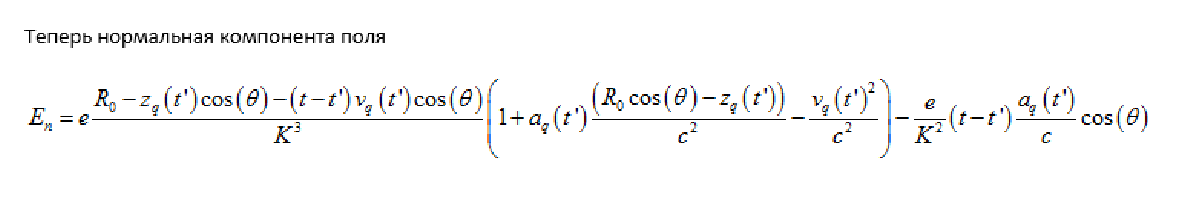
\includegraphics[keepaspectratio,totalheight=10.472222222222221in,angle=-90]{gauss_theorem_with_acceleration_piecewiceimage5.eps}}}\end{Maple Normal}
}\end{Maple Normal}
\begin{Maple Normal}{
\begin{Maple Normal}{
}\end{Maple Normal}
}\end{Maple Normal}
\begin{Maple Normal}{
\begin{Maple Normal}{
\mapleinline{inert}{2d}{Enf := proc (T, Theta) options operator, arrow; subs(z__0 = Z, v__0 = V, a__0 = A, c = 1, R__0 = R, tau__0 = Tau__0, (R__0-z__q(z__0, v__0, a__0, ftau(T, Theta), tau__0)*cos(Theta)-(T-ftau(T, Theta))*v__q(v__0, a__0, ftau(T, Theta), tau__0)*cos(Theta))*(1+a__q(a__0, ftau(T, Theta), tau__0)*(R__0*cos(Theta)-z__q(z__0, v__0, a__0, ftau(T, Theta), tau__0))/c^2-v__q(v__0, a__0, ftau(T, Theta), tau__0)^2/c^2)/Rlwf(T, Theta)^3-(T-ftau(T, Theta))*a__q(a__0, ftau(T, Theta), tau__0)*cos(Theta)/(c*Rlwf(T, Theta)^2)) end proc}{\[\displaystyle {\it Enf}\, := \,( {T,\Theta} )\mapsto {\frac { \left( R-z_{q} \left( Z,V,A,{\it ftau} \left( T,\Theta \right) ,{\it Tau}_{0} \right) \cos \left( \Theta \right) \\
\mbox{}- \left( T-{\it ftau} \left( T,\Theta \right)  \right) v_{q} \left( V,A,{\it ftau} \left( T,\Theta \right) ,{\it Tau}_{0} \right) \cos \left( \Theta \right)  \right)  \left( 1+a_{q} \left( A,{\it ftau} \left( T,\Theta \right) ,{\it Tau}_{0} \right)  \left( R\cos \left( \Theta \right) -z_{q} \left( Z,V,A,{\it ftau} \left( T,\Theta \right) ,{\it Tau}_{0} \right)  \right) - \left( v_{q} \left( V,A,{\it ftau} \left( T,\Theta \right) ,{\it Tau}_{0} \right)  \right) ^{2} \right) \\
\mbox{}}{ \left( {\it Rlwf} \left( T,\Theta \right)  \right) ^{3}}}-{\frac { \left( T-{\it ftau} \left( T,\Theta \right)  \right) a_{q} \left( A,{\it ftau} \left( T,\Theta \right) ,{\it Tau}_{0} \right) \cos \left( \Theta \right) }{ \left( {\it Rlwf} \left( T,\Theta \right)  \right) ^{2}}}\]}
}\end{Maple Normal}
\begin{Maple Normal}{
\mapleinline{inert}{2d}{Enf := proc (T, Theta) options operator, arrow; subs(z__0 = Z, v__0 = V, a__0 = A, c = 1, R__0 = R, tau__0 = Tau__0, (R__0-z__q(z__0, v__0, a__0, ftau(T, Theta), tau__0)*cos(Theta)-(T-ftau(T, Theta))*v__q(v__0, a__0, ftau(T, Theta), tau__0)*cos(Theta))*(1+a__q(a__0, ftau(T, Theta), tau__0)*(R__0*cos(Theta)-z__q(z__0, v__0, a__0, ftau(T, Theta), tau__0))/c^2-v__q(v__0, a__0, ftau(T, Theta), tau__0)^2/c^2)/Rlwf(T, Theta)^3-(T-ftau(T, Theta))*a__q(a__0, ftau(T, Theta), tau__0)*cos(Theta)/(c*Rlwf(T, Theta)^2)) end proc}{\[\displaystyle {\it Enf}\, := \,( {T,\Theta} )\mapsto {\frac { \left( R-z_{q} \left( Z,V,A,{\it ftau} \left( T,\Theta \right) ,{\it Tau}_{0} \right) \cos \left( \Theta \right) \\
\mbox{}- \left( T-{\it ftau} \left( T,\Theta \right)  \right) v_{q} \left( V,A,{\it ftau} \left( T,\Theta \right) ,{\it Tau}_{0} \right) \cos \left( \Theta \right)  \right)  \left( 1+a_{q} \left( A,{\it ftau} \left( T,\Theta \right) ,{\it Tau}_{0} \right)  \left( R\cos \left( \Theta \right) -z_{q} \left( Z,V,A,{\it ftau} \left( T,\Theta \right) ,{\it Tau}_{0} \right)  \right) - \left( v_{q} \left( V,A,{\it ftau} \left( T,\Theta \right) ,{\it Tau}_{0} \right)  \right) ^{2} \right) \\
\mbox{}}{ \left( {\it Rlwf} \left( T,\Theta \right)  \right) ^{3}}}-{\frac { \left( T-{\it ftau} \left( T,\Theta \right)  \right) a_{q} \left( A,{\it ftau} \left( T,\Theta \right) ,{\it Tau}_{0} \right) \cos \left( \Theta \right) }{ \left( {\it Rlwf} \left( T,\Theta \right)  \right) ^{2}}}\]}
}\end{Maple Normal}
\begin{Maple Normal}{
\mapleinline{inert}{2d}{Enf := proc (T, Theta) options operator, arrow; subs(z__0 = Z, v__0 = V, a__0 = A, c = 1, R__0 = R, tau__0 = Tau__0, (R__0-z__q(z__0, v__0, a__0, ftau(T, Theta), tau__0)*cos(Theta)-(T-ftau(T, Theta))*v__q(v__0, a__0, ftau(T, Theta), tau__0)*cos(Theta))*(1+a__q(a__0, ftau(T, Theta), tau__0)*(R__0*cos(Theta)-z__q(z__0, v__0, a__0, ftau(T, Theta), tau__0))/c^2-v__q(v__0, a__0, ftau(T, Theta), tau__0)^2/c^2)/Rlwf(T, Theta)^3-(T-ftau(T, Theta))*a__q(a__0, ftau(T, Theta), tau__0)*cos(Theta)/(c*Rlwf(T, Theta)^2)) end proc}{\[\displaystyle {\it Enf}\, := \,( {T,\Theta} )\mapsto {\frac { \left( R-z_{q} \left( Z,V,A,{\it ftau} \left( T,\Theta \right) ,{\it Tau}_{0} \right) \cos \left( \Theta \right) \\
\mbox{}- \left( T-{\it ftau} \left( T,\Theta \right)  \right) v_{q} \left( V,A,{\it ftau} \left( T,\Theta \right) ,{\it Tau}_{0} \right) \cos \left( \Theta \right)  \right)  \left( 1+a_{q} \left( A,{\it ftau} \left( T,\Theta \right) ,{\it Tau}_{0} \right)  \left( R\cos \left( \Theta \right) -z_{q} \left( Z,V,A,{\it ftau} \left( T,\Theta \right) ,{\it Tau}_{0} \right)  \right) - \left( v_{q} \left( V,A,{\it ftau} \left( T,\Theta \right) ,{\it Tau}_{0} \right)  \right) ^{2} \right) \\
\mbox{}}{ \left( {\it Rlwf} \left( T,\Theta \right)  \right) ^{3}}}-{\frac { \left( T-{\it ftau} \left( T,\Theta \right)  \right) a_{q} \left( A,{\it ftau} \left( T,\Theta \right) ,{\it Tau}_{0} \right) \cos \left( \Theta \right) }{ \left( {\it Rlwf} \left( T,\Theta \right)  \right) ^{2}}}\]}
}\end{Maple Normal}
}\end{Maple Normal}
\begin{maplegroup}
\begin{Maple Normal}{
\mapleinline{inert}{2d}{Enf := proc (T, Theta) options operator, arrow; subs(z__0 = Z, v__0 = V, a__0 = A, c = 1, R__0 = R, tau__0 = Tau__0, (R__0-z__q(z__0, v__0, a__0, ftau(T, Theta), tau__0)*cos(Theta)-(T-ftau(T, Theta))*v__q(v__0, a__0, ftau(T, Theta), tau__0)*cos(Theta))*(1+a__q(a__0, ftau(T, Theta), tau__0)*(R__0*cos(Theta)-z__q(z__0, v__0, a__0, ftau(T, Theta), tau__0))/c^2-v__q(v__0, a__0, ftau(T, Theta), tau__0)^2/c^2)/Rlwf(T, Theta)^3-(T-ftau(T, Theta))*a__q(a__0, ftau(T, Theta), tau__0)*cos(Theta)/(c*Rlwf(T, Theta)^2)) end proc}{\[\displaystyle {\it Enf}\, := \,( {T,\Theta} )\mapsto {\frac { \left( R-z_{q} \left( Z,V,A,{\it ftau} \left( T,\Theta \right) ,{\it Tau}_{0} \right) \cos \left( \Theta \right) \\
\mbox{}- \left( T-{\it ftau} \left( T,\Theta \right)  \right) v_{q} \left( V,A,{\it ftau} \left( T,\Theta \right) ,{\it Tau}_{0} \right) \cos \left( \Theta \right)  \right)  \left( 1+a_{q} \left( A,{\it ftau} \left( T,\Theta \right) ,{\it Tau}_{0} \right)  \left( R\cos \left( \Theta \right) -z_{q} \left( Z,V,A,{\it ftau} \left( T,\Theta \right) ,{\it Tau}_{0} \right)  \right) - \left( v_{q} \left( V,A,{\it ftau} \left( T,\Theta \right) ,{\it Tau}_{0} \right)  \right) ^{2} \right) \\
\mbox{}}{ \left( {\it Rlwf} \left( T,\Theta \right)  \right) ^{3}}}-{\frac { \left( T-{\it ftau} \left( T,\Theta \right)  \right) a_{q} \left( A,{\it ftau} \left( T,\Theta \right) ,{\it Tau}_{0} \right) \cos \left( \Theta \right) }{ \left( {\it Rlwf} \left( T,\Theta \right)  \right) ^{2}}}\]}
}\end{Maple Normal}
\mapleresult
\begin{maplelatex}
\mapleinline{inert}{2d}{proc (T, Theta) options operator, arrow; subs(z__0 = Z, v__0 = V, a__0 = A, c = 1, R__0 = R, tau__0 = Tau__0, (R__0-z__q(z__0, v__0, a__0, ftau(T, Theta), tau__0)*cos(Theta)-(T-ftau(T, Theta))*v__q(v__0, a__0, ftau(T, Theta), tau__0)*cos(Theta))*(1+a__q(a__0, ftau(T, Theta), tau__0)*(R__0*cos(Theta)-z__q(z__0, v__0, a__0, ftau(T, Theta), tau__0))/c^2-v__q(v__0, a__0, ftau(T, Theta), tau__0)^2/c^2)/Rlwf(T, Theta)^3-(T-ftau(T, Theta))*a__q(a__0, ftau(T, Theta), tau__0)*cos(Theta)/(c*Rlwf(T, Theta)^2)) end proc}{\[\displaystyle ( {T,\Theta} )\mapsto {\frac { \left( R-z_{q} \left( Z,V,A,{\it ftau} \left( T,\Theta \right) ,{\it Tau}_{0} \right) \cos \left( \Theta \right) \\
\mbox{}- \left( T-{\it ftau} \left( T,\Theta \right)  \right) v_{q} \left( V,A,{\it ftau} \left( T,\Theta \right) ,{\it Tau}_{0} \right) \cos \left( \Theta \right)  \right)  \left( 1+a_{q} \left( A,{\it ftau} \left( T,\Theta \right) ,{\it Tau}_{0} \right)  \left( R\cos \left( \Theta \right) -z_{q} \left( Z,V,A,{\it ftau} \left( T,\Theta \right) ,{\it Tau}_{0} \right)  \right) - \left( v_{q} \left( V,A,{\it ftau} \left( T,\Theta \right) ,{\it Tau}_{0} \right)  \right) ^{2} \right) \\
\mbox{}}{ \left( {\it Rlwf} \left( T,\Theta \right)  \right) ^{3}}}-{\frac { \left( T-{\it ftau} \left( T,\Theta \right)  \right) a_{q} \left( A,{\it ftau} \left( T,\Theta \right) ,{\it Tau}_{0} \right) \cos \left( \Theta \right) }{ \left( {\it Rlwf} \left( T,\Theta \right)  \right) ^{2}}}\]}
\end{maplelatex}
\end{maplegroup}
\begin{Maple Normal}{
\begin{Maple Normal}{
}\end{Maple Normal}
}\end{Maple Normal}
\begin{Maple Normal}{
\begin{Maple Normal}{
\mapleinline{inert}{2d}{Enr := proc (T, Theta) options operator, arrow; subs(z__0 = Z, v__0 = V, a__0 = A, c = 1, R__0 = R, tau__0 = Tau__0, (R__0-z__q(z__0, v__0, a__0, rtau(T, Theta), tau__0)*cos(Theta)-(T-rtau(T, Theta))*v__q(v__0, a__0, rtau(T, Theta), tau__0)*cos(Theta))*(1+a__q(a__0, rtau(T, Theta), tau__0)*(R__0*cos(Theta)-z__q(z__0, v__0, a__0, rtau(T, Theta), tau__0))/c^2-v__q(v__0, a__0, rtau(T, Theta), tau__0)^2/c^2)/Rlwr(T, Theta)^3-(T-rtau(T, Theta))*a__q(a__0, rtau(T, Theta), tau__0)*cos(Theta)/(c*Rlwr(T, Theta)^2)) end proc}{\[\displaystyle {\it Enr}\, := \,( {T,\Theta} )\mapsto {\frac { \left( R-z_{q} \left( Z,V,A,{\it rtau} \left( T,\Theta \right) ,{\it Tau}_{0} \right) \cos \left( \Theta \right) \\
\mbox{}- \left( T-{\it rtau} \left( T,\Theta \right)  \right) v_{q} \left( V,A,{\it rtau} \left( T,\Theta \right) ,{\it Tau}_{0} \right) \cos \left( \Theta \right)  \right)  \left( 1+a_{q} \left( A,{\it rtau} \left( T,\Theta \right) ,{\it Tau}_{0} \right)  \left( R\cos \left( \Theta \right) -z_{q} \left( Z,V,A,{\it rtau} \left( T,\Theta \right) ,{\it Tau}_{0} \right)  \right) - \left( v_{q} \left( V,A,{\it rtau} \left( T,\Theta \right) ,{\it Tau}_{0} \right)  \right) ^{2} \right) \\
\mbox{}}{ \left( {\it Rlwr} \left( T,\Theta \right)  \right) ^{3}}}-{\frac { \left( T-{\it rtau} \left( T,\Theta \right)  \right) a_{q} \left( A,{\it rtau} \left( T,\Theta \right) ,{\it Tau}_{0} \right) \cos \left( \Theta \right) }{ \left( {\it Rlwr} \left( T,\Theta \right)  \right) ^{2}}}\]}
}\end{Maple Normal}
\begin{Maple Normal}{
\mapleinline{inert}{2d}{Enr := proc (T, Theta) options operator, arrow; subs(z__0 = Z, v__0 = V, a__0 = A, c = 1, R__0 = R, tau__0 = Tau__0, (R__0-z__q(z__0, v__0, a__0, rtau(T, Theta), tau__0)*cos(Theta)-(T-rtau(T, Theta))*v__q(v__0, a__0, rtau(T, Theta), tau__0)*cos(Theta))*(1+a__q(a__0, rtau(T, Theta), tau__0)*(R__0*cos(Theta)-z__q(z__0, v__0, a__0, rtau(T, Theta), tau__0))/c^2-v__q(v__0, a__0, rtau(T, Theta), tau__0)^2/c^2)/Rlwr(T, Theta)^3-(T-rtau(T, Theta))*a__q(a__0, rtau(T, Theta), tau__0)*cos(Theta)/(c*Rlwr(T, Theta)^2)) end proc}{\[\displaystyle {\it Enr}\, := \,( {T,\Theta} )\mapsto {\frac { \left( R-z_{q} \left( Z,V,A,{\it rtau} \left( T,\Theta \right) ,{\it Tau}_{0} \right) \cos \left( \Theta \right) \\
\mbox{}- \left( T-{\it rtau} \left( T,\Theta \right)  \right) v_{q} \left( V,A,{\it rtau} \left( T,\Theta \right) ,{\it Tau}_{0} \right) \cos \left( \Theta \right)  \right)  \left( 1+a_{q} \left( A,{\it rtau} \left( T,\Theta \right) ,{\it Tau}_{0} \right)  \left( R\cos \left( \Theta \right) -z_{q} \left( Z,V,A,{\it rtau} \left( T,\Theta \right) ,{\it Tau}_{0} \right)  \right) - \left( v_{q} \left( V,A,{\it rtau} \left( T,\Theta \right) ,{\it Tau}_{0} \right)  \right) ^{2} \right) \\
\mbox{}}{ \left( {\it Rlwr} \left( T,\Theta \right)  \right) ^{3}}}-{\frac { \left( T-{\it rtau} \left( T,\Theta \right)  \right) a_{q} \left( A,{\it rtau} \left( T,\Theta \right) ,{\it Tau}_{0} \right) \cos \left( \Theta \right) }{ \left( {\it Rlwr} \left( T,\Theta \right)  \right) ^{2}}}\]}
}\end{Maple Normal}
}\end{Maple Normal}
\begin{maplegroup}
\begin{Maple Normal}{
\mapleinline{inert}{2d}{Enr := proc (T, Theta) options operator, arrow; subs(z__0 = Z, v__0 = V, a__0 = A, c = 1, R__0 = R, tau__0 = Tau__0, (R__0-z__q(z__0, v__0, a__0, rtau(T, Theta), tau__0)*cos(Theta)-(T-rtau(T, Theta))*v__q(v__0, a__0, rtau(T, Theta), tau__0)*cos(Theta))*(1+a__q(a__0, rtau(T, Theta), tau__0)*(R__0*cos(Theta)-z__q(z__0, v__0, a__0, rtau(T, Theta), tau__0))/c^2-v__q(v__0, a__0, rtau(T, Theta), tau__0)^2/c^2)/Rlwr(T, Theta)^3-(T-rtau(T, Theta))*a__q(a__0, rtau(T, Theta), tau__0)*cos(Theta)/(c*Rlwr(T, Theta)^2)) end proc}{\[\displaystyle {\it Enr}\, := \,( {T,\Theta} )\mapsto {\frac { \left( R-z_{q} \left( Z,V,A,{\it rtau} \left( T,\Theta \right) ,{\it Tau}_{0} \right) \cos \left( \Theta \right) \\
\mbox{}- \left( T-{\it rtau} \left( T,\Theta \right)  \right) v_{q} \left( V,A,{\it rtau} \left( T,\Theta \right) ,{\it Tau}_{0} \right) \cos \left( \Theta \right)  \right)  \left( 1+a_{q} \left( A,{\it rtau} \left( T,\Theta \right) ,{\it Tau}_{0} \right)  \left( R\cos \left( \Theta \right) -z_{q} \left( Z,V,A,{\it rtau} \left( T,\Theta \right) ,{\it Tau}_{0} \right)  \right) - \left( v_{q} \left( V,A,{\it rtau} \left( T,\Theta \right) ,{\it Tau}_{0} \right)  \right) ^{2} \right) \\
\mbox{}}{ \left( {\it Rlwr} \left( T,\Theta \right)  \right) ^{3}}}-{\frac { \left( T-{\it rtau} \left( T,\Theta \right)  \right) a_{q} \left( A,{\it rtau} \left( T,\Theta \right) ,{\it Tau}_{0} \right) \cos \left( \Theta \right) }{ \left( {\it Rlwr} \left( T,\Theta \right)  \right) ^{2}}}\]}
}\end{Maple Normal}
\mapleresult
\begin{maplelatex}
\mapleinline{inert}{2d}{proc (T, Theta) options operator, arrow; subs(z__0 = Z, v__0 = V, a__0 = A, c = 1, R__0 = R, tau__0 = Tau__0, (R__0-z__q(z__0, v__0, a__0, rtau(T, Theta), tau__0)*cos(Theta)-(T-rtau(T, Theta))*v__q(v__0, a__0, rtau(T, Theta), tau__0)*cos(Theta))*(1+a__q(a__0, rtau(T, Theta), tau__0)*(R__0*cos(Theta)-z__q(z__0, v__0, a__0, rtau(T, Theta), tau__0))/c^2-v__q(v__0, a__0, rtau(T, Theta), tau__0)^2/c^2)/Rlwr(T, Theta)^3-(T-rtau(T, Theta))*a__q(a__0, rtau(T, Theta), tau__0)*cos(Theta)/(c*Rlwr(T, Theta)^2)) end proc}{\[\displaystyle ( {T,\Theta} )\mapsto {\frac { \left( R-z_{q} \left( Z,V,A,{\it rtau} \left( T,\Theta \right) ,{\it Tau}_{0} \right) \cos \left( \Theta \right) \\
\mbox{}- \left( T-{\it rtau} \left( T,\Theta \right)  \right) v_{q} \left( V,A,{\it rtau} \left( T,\Theta \right) ,{\it Tau}_{0} \right) \cos \left( \Theta \right)  \right)  \left( 1+a_{q} \left( A,{\it rtau} \left( T,\Theta \right) ,{\it Tau}_{0} \right)  \left( R\cos \left( \Theta \right) -z_{q} \left( Z,V,A,{\it rtau} \left( T,\Theta \right) ,{\it Tau}_{0} \right)  \right) - \left( v_{q} \left( V,A,{\it rtau} \left( T,\Theta \right) ,{\it Tau}_{0} \right)  \right) ^{2} \right) \\
\mbox{}}{ \left( {\it Rlwr} \left( T,\Theta \right)  \right) ^{3}}}-{\frac { \left( T-{\it rtau} \left( T,\Theta \right)  \right) a_{q} \left( A,{\it rtau} \left( T,\Theta \right) ,{\it Tau}_{0} \right) \cos \left( \Theta \right) }{ \left( {\it Rlwr} \left( T,\Theta \right)  \right) ^{2}}}\]}
\end{maplelatex}
\end{maplegroup}
\begin{Maple Normal}{
\begin{Maple Normal}{
}\end{Maple Normal}
}\end{Maple Normal}
\begin{Maple Normal}{
\begin{Maple Normal}{
}\end{Maple Normal}
}\end{Maple Normal}
\begin{Maple Normal}{
\begin{Maple Normal}{
\mapleinline{inert}{2d}{evalf(Enf(2, 0))}{\[\displaystyle {\it evalf} \left( {\it Enf} \left( 2,0 \right)  \right) \]}
}\end{Maple Normal}
}\end{Maple Normal}
\begin{maplegroup}
\begin{Maple Normal}{
\mapleinline{inert}{2d}{evalf(Enf(2, 0))}{\[\displaystyle {\it evalf} \left( {\it Enf} \left( 2,0 \right)  \right) \]}
}\end{Maple Normal}
\mapleresult
\begin{maplelatex}
\mapleinline{inert}{2d}{1.386271243}{\[\displaystyle  1.386271243\]}
\end{maplelatex}
\end{maplegroup}
\begin{Maple Normal}{
\begin{Maple Normal}{
\mapleinline{inert}{2d}{evalf(Enr(2, 0))}{\[\displaystyle {\it evalf} \left( {\it Enr} \left( 2,0 \right)  \right) \]}
}\end{Maple Normal}
}\end{Maple Normal}
\begin{maplegroup}
\begin{Maple Normal}{
\mapleinline{inert}{2d}{evalf(Enr(2, 0))}{\[\displaystyle {\it evalf} \left( {\it Enr} \left( 2,0 \right)  \right) \]}
}\end{Maple Normal}
\mapleresult
\begin{maplelatex}
\mapleinline{inert}{2d}{1.386271243}{\[\displaystyle  1.386271243\]}
\end{maplelatex}
\end{maplegroup}
\begin{Maple Normal}{
\begin{Maple Normal}{
}\end{Maple Normal}
}\end{Maple Normal}
\begin{Maple Normal}{
\begin{Maple Normal}{
}\end{Maple Normal}
}\end{Maple Normal}
\begin{Maple Normal}{
\begin{Maple Normal}{
\mapleinline{inert}{2d}{plot3d('Enf(T, Theta)', Theta = 0 .. Pi, T = 0 .. 3)}{\[\displaystyle {\it plot3d} \left( '\mathit{Enf} (T,\,Theta)',\Theta={0\ldots \pi},T={0\ldots 3}\\
\mbox{} \right) \]}
}\end{Maple Normal}
}\end{Maple Normal}
\begin{maplegroup}
\begin{Maple Normal}{
\mapleinline{inert}{2d}{plot3d('Enf(T, Theta)', Theta = 0 .. Pi, T = 0 .. 3)}{\[\displaystyle {\it plot3d} \left( '\mathit{Enf} (T,\,Theta)',\Theta={0\ldots \pi},T={0\ldots 3}\\
\mbox{} \right) \]}
}\end{Maple Normal}
\mapleresult
\mapleplot{gauss_theorem_with_acceleration_piecewiceplot3d5.eps}
\end{maplegroup}
\begin{Maple Normal}{
\begin{Maple Normal}{
}\end{Maple Normal}
}\end{Maple Normal}
\begin{Maple Normal}{
\begin{Maple Normal}{
\mapleinline{inert}{2d}{plot3d('Enf(T, Theta)*sin(Theta)', Theta = 0 .. Pi, T = 0 .. 3)}{\[\displaystyle {\it plot3d} \left( '\mathit{Enf} (T,\,Theta) \ast \mathit{sin} (Theta)',\Theta={0\ldots \pi},T={0\ldots 3}\\
\mbox{} \right) \]}
}\end{Maple Normal}
}\end{Maple Normal}
\begin{maplegroup}
\begin{Maple Normal}{
\mapleinline{inert}{2d}{plot3d('Enf(T, Theta)*sin(Theta)', Theta = 0 .. Pi, T = 0 .. 3)}{\[\displaystyle {\it plot3d} \left( '\mathit{Enf} (T,\,Theta) \ast \mathit{sin} (Theta)',\Theta={0\ldots \pi},T={0\ldots 3}\\
\mbox{} \right) \]}
}\end{Maple Normal}
\mapleresult
\mapleplot{gauss_theorem_with_acceleration_piecewiceplot3d6.eps}
\end{maplegroup}
\begin{Maple Normal}{
\begin{Maple Normal}{
\mapleinline{inert}{2d}{plot('Enf(3, Theta)', Theta = 0 .. Pi)}{\[\displaystyle {\it plot} \left( '\mathit{Enf} (3,\,Theta)',\Theta={0\ldots \pi} \right) \]}
}\end{Maple Normal}
}\end{Maple Normal}
\begin{maplegroup}
\begin{Maple Normal}{
\mapleinline{inert}{2d}{plot('Enf(3, Theta)', Theta = 0 .. Pi)}{\[\displaystyle {\it plot} \left( '\mathit{Enf} (3,\,Theta)',\Theta={0\ldots \pi} \right) \]}
}\end{Maple Normal}
\mapleresult
\mapleplot{gauss_theorem_with_acceleration_piecewiceplot2d7.eps}
\end{maplegroup}
\begin{Maple Normal}{
\begin{Maple Normal}{
\mapleinline{inert}{2d}{plot('Enr(3, Theta)', Theta = 0 .. Pi)}{\[\displaystyle {\it plot} \left( '\mathit{Enr} (3,\,Theta)',\Theta={0\ldots \pi} \right) \]}
}\end{Maple Normal}
}\end{Maple Normal}
\begin{maplegroup}
\begin{Maple Normal}{
\mapleinline{inert}{2d}{plot('Enr(3, Theta)', Theta = 0 .. Pi)}{\[\displaystyle {\it plot} \left( '\mathit{Enr} (3,\,Theta)',\Theta={0\ldots \pi} \right) \]}
}\end{Maple Normal}
\mapleresult
\mapleplot{gauss_theorem_with_acceleration_piecewiceplot2d8.eps}
\end{maplegroup}
\begin{Maple Normal}{
\begin{Maple Normal}{
}\end{Maple Normal}
}\end{Maple Normal}
\begin{Maple Normal}{
\begin{Maple Normal}{
}\end{Maple Normal}
}\end{Maple Normal}
\begin{Maple Normal}{
\begin{Maple Normal}{
\mapleinline{inert}{2d}{plot('Enf(3, Theta)*sin(Theta)', Theta = 0 .. Pi)}{\[\displaystyle {\it plot} \left( '\mathit{Enf} (3,\,Theta) \ast \mathit{sin} (Theta)',\Theta={0\ldots \pi} \right) \]}
}\end{Maple Normal}
}\end{Maple Normal}
\begin{maplegroup}
\begin{Maple Normal}{
\mapleinline{inert}{2d}{plot('Enf(3, Theta)*sin(Theta)', Theta = 0 .. Pi)}{\[\displaystyle {\it plot} \left( '\mathit{Enf} (3,\,Theta) \ast \mathit{sin} (Theta)',\Theta={0\ldots \pi} \right) \]}
}\end{Maple Normal}
\mapleresult
\mapleplot{gauss_theorem_with_acceleration_piecewiceplot2d9.eps}
\end{maplegroup}
\begin{Maple Normal}{
\begin{Maple Normal}{
\mapleinline{inert}{2d}{plot(([seq])(eval(Enr(T, Theta), T = t), t = 0 .. 3), Theta = 0 .. Pi)}{\[\displaystyle {\it plot} \left( [{\it seq}] \left( {\it eval} \left( {\it Enr} \left( T\\
\mbox{},\Theta \right) ,T\\
\mbox{}=t \right) ,t={0\ldots 3} \right) ,\Theta={0\ldots \pi} \right) \]}
}\end{Maple Normal}
\begin{Maple Normal}{
\mapleinline{inert}{2d}{plot(([seq])(eval(Enr(T, Theta), T = t), t = 0 .. 3), Theta = 0 .. Pi)}{\[\displaystyle {\it plot} \left( [{\it seq}] \left( {\it eval} \left( {\it Enr} \left( T\\
\mbox{},\Theta \right) ,T\\
\mbox{}=t \right) ,t={0\ldots 3} \right) ,\Theta={0\ldots \pi} \right) \]}
}\end{Maple Normal}
}\end{Maple Normal}
\begin{maplegroup}
\begin{Maple Normal}{
\mapleinline{inert}{2d}{plot(([seq])(eval(Enr(T, Theta), T = t), t = 0 .. 3), Theta = 0 .. Pi)}{\[\displaystyle {\it plot} \left( [{\it seq}] \left( {\it eval} \left( {\it Enr} \left( T\\
\mbox{},\Theta \right) ,T\\
\mbox{}=t \right) ,t={0\ldots 3} \right) ,\Theta={0\ldots \pi} \right) \]}
}\end{Maple Normal}
\mapleresult
\mapleplot{gauss_theorem_with_acceleration_piecewiceplot2d10.eps}
\end{maplegroup}
\begin{Maple Normal}{
\begin{Maple Normal}{
\mapleinline{inert}{2d}{plot(([seq])(eval(Enr(T, Theta)*sin(Theta), T = t), t = 0 .. 3), Theta = 0 .. Pi)}{\[\displaystyle {\it plot} \left( [{\it seq}] \left( {\it eval} \left( {\it Enr} \left( T,\Theta \right) \\
\mbox{}\sin \left( \Theta \right) ,T=t \right) ,t={0\ldots 3} \right) ,\Theta={0\ldots \pi} \right) \]}
}\end{Maple Normal}
}\end{Maple Normal}
\begin{maplegroup}
\begin{Maple Normal}{
\mapleinline{inert}{2d}{plot(([seq])(eval(Enr(T, Theta)*sin(Theta), T = t), t = 0 .. 3), Theta = 0 .. Pi)}{\[\displaystyle {\it plot} \left( [{\it seq}] \left( {\it eval} \left( {\it Enr} \left( T,\Theta \right) \\
\mbox{}\sin \left( \Theta \right) ,T=t \right) ,t={0\ldots 3} \right) ,\Theta={0\ldots \pi} \right) \]}
}\end{Maple Normal}
\mapleresult
\mapleplot{gauss_theorem_with_acceleration_piecewiceplot2d11.eps}
\end{maplegroup}
\begin{Maple Normal}{
\begin{Maple Normal}{
}\end{Maple Normal}
}\end{Maple Normal}
\begin{Maple Normal}{
\begin{Maple Normal}{
}\end{Maple Normal}
}\end{Maple Normal}
\begin{Maple Normal}{
\begin{Maple Normal}{
\mapleinline{inert}{2d}{k := proc (T) options operator, arrow; evalf(Int(Enr(T, Theta)*R^2*sin(Theta), Theta = 0 .. Pi)) end proc}{\[\displaystyle k\, := \,T\mapsto \int_{ 0.0}^{ 3.141592654}\!{\it Enr} \left( T,\Theta \right) \\
\mbox{}{R}^{2}\sin \left( \Theta \right) \,{\rm d}\Theta\]}
}\end{Maple Normal}
\begin{Maple Normal}{
\mapleinline{inert}{2d}{k := proc (T) options operator, arrow; evalf(Int(Enr(T, Theta)*R^2*sin(Theta), Theta = 0 .. Pi)) end proc}{\[\displaystyle k\, := \,T\mapsto \int_{ 0.0}^{ 3.141592654}\!{\it Enr} \left( T,\Theta \right) \\
\mbox{}{R}^{2}\sin \left( \Theta \right) \,{\rm d}\Theta\]}
}\end{Maple Normal}
}\end{Maple Normal}
\begin{maplegroup}
\begin{Maple Normal}{
\mapleinline{inert}{2d}{k := proc (T) options operator, arrow; evalf(Int(Enr(T, Theta)*R^2*sin(Theta), Theta = 0 .. Pi)) end proc}{\[\displaystyle k\, := \,T\mapsto \int_{ 0.0}^{ 3.141592654}\!{\it Enr} \left( T,\Theta \right) \\
\mbox{}{R}^{2}\sin \left( \Theta \right) \,{\rm d}\Theta\]}
}\end{Maple Normal}
\mapleresult
\begin{maplelatex}
\mapleinline{inert}{2d}{proc (T) options operator, arrow; evalf(Int(Enr(T, Theta)*R^2*sin(Theta), Theta = 0 .. Pi)) end proc}{\[\displaystyle T\mapsto \int_{ 0.0}^{ 3.141592654}\!{\it Enr} \left( T,\Theta \right) \\
\mbox{}{R}^{2}\sin \left( \Theta \right) \,{\rm d}\Theta\]}
\end{maplelatex}
\end{maplegroup}
\begin{Maple Normal}{
\begin{Maple Normal}{
\mapleinline{inert}{2d}{evalf(k(0))}{\[\displaystyle {\it evalf} \left( k \left( 0 \right)  \right) \]}
}\end{Maple Normal}
}\end{Maple Normal}
\begin{maplegroup}
\begin{Maple Normal}{
\mapleinline{inert}{2d}{evalf(k(0))}{\[\displaystyle {\it evalf} \left( k \left( 0 \right)  \right) \]}
}\end{Maple Normal}
\mapleresult
\begin{maplelatex}
\mapleinline{inert}{2d}{2.000000000}{\[\displaystyle  2.0\]}
\end{maplelatex}
\end{maplegroup}
\begin{Maple Normal}{
\begin{Maple Normal}{
\mapleinline{inert}{2d}{evalf(k(1))}{\[\displaystyle {\it evalf} \left( k \left( 1 \right)  \right) \]}
}\end{Maple Normal}
}\end{Maple Normal}
\begin{maplegroup}
\begin{Maple Normal}{
\mapleinline{inert}{2d}{evalf(k(1))}{\[\displaystyle {\it evalf} \left( k \left( 1 \right)  \right) \]}
}\end{Maple Normal}
\mapleresult
\begin{maplelatex}
\mapleinline{inert}{2d}{2.000000000}{\[\displaystyle  2.0\]}
\end{maplelatex}
\end{maplegroup}
\begin{Maple Normal}{
\begin{Maple Normal}{
\mapleinline{inert}{2d}{evalf(k(2))}{\[\displaystyle {\it evalf} \left( k \left( 2 \right)  \right) \]}
}\end{Maple Normal}
}\end{Maple Normal}
\begin{maplegroup}
\begin{Maple Normal}{
\mapleinline{inert}{2d}{evalf(k(2))}{\[\displaystyle {\it evalf} \left( k \left( 2 \right)  \right) \]}
}\end{Maple Normal}
\mapleresult
\begin{maplelatex}
\mapleinline{inert}{2d}{2.015336698}{\[\displaystyle  2.015336698\]}
\end{maplelatex}
\end{maplegroup}
\begin{Maple Normal}{
\begin{Maple Normal}{
\mapleinline{inert}{2d}{evalf(k(3))}{\[\displaystyle {\it evalf} \left( k \left( 3 \right)  \right) \]}
}\end{Maple Normal}
}\end{Maple Normal}
\begin{maplegroup}
\begin{Maple Normal}{
\mapleinline{inert}{2d}{evalf(k(3))}{\[\displaystyle {\it evalf} \left( k \left( 3 \right)  \right) \]}
}\end{Maple Normal}
\mapleresult
\begin{maplelatex}
\mapleinline{inert}{2d}{2.189712498}{\[\displaystyle  2.189712498\]}
\end{maplelatex}
\end{maplegroup}
\begin{Maple Normal}{
\begin{Maple Normal}{
\mapleinline{inert}{2d}{evalf(k(4))}{\[\displaystyle {\it evalf} \left( k \left( 4 \right)  \right) \]}
}\end{Maple Normal}
}\end{Maple Normal}
\begin{maplegroup}
\begin{Maple Normal}{
\mapleinline{inert}{2d}{evalf(k(4))}{\[\displaystyle {\it evalf} \left( k \left( 4 \right)  \right) \]}
}\end{Maple Normal}
\mapleresult
\begin{maplelatex}
\mapleinline{inert}{2d}{3.594958824}{\[\displaystyle  3.594958824\]}
\end{maplelatex}
\end{maplegroup}
\begin{Maple Normal}{
\begin{Maple Normal}{
\mapleinline{inert}{2d}{evalf(k(5))}{\[\displaystyle {\it evalf} \left( k \left( 5 \right)  \right) \]}
}\end{Maple Normal}
}\end{Maple Normal}
\begin{maplegroup}
\begin{Maple Normal}{
\mapleinline{inert}{2d}{evalf(k(5))}{\[\displaystyle {\it evalf} \left( k \left( 5 \right)  \right) \]}
}\end{Maple Normal}
\mapleresult
\begin{maplelatex}
\mapleinline{inert}{2d}{6.429266743}{\[\displaystyle  6.429266743\]}
\end{maplelatex}
\end{maplegroup}
\begin{Maple Normal}{
\begin{Maple Normal}{
\mapleinline{inert}{2d}{plot(k(T), T = 0 .. 4)}{\[\displaystyle {\it plot} \left( k \left( T \right) ,T={0\ldots 4} \right) \]}
}\end{Maple Normal}
}\end{Maple Normal}
\begin{maplegroup}
\begin{Maple Normal}{
\mapleinline{inert}{2d}{plot(k(T), T = 0 .. 4)}{\[\displaystyle {\it plot} \left( k \left( T \right) ,T={0\ldots 4} \right) \]}
}\end{Maple Normal}
\mapleresult
\mapleplot{gauss_theorem_with_acceleration_piecewiceplot2d12.eps}
\end{maplegroup}
\begin{Maple Normal}{
\begin{Maple Normal}{
}\end{Maple Normal}
}\end{Maple Normal}
\begin{Maple Normal}{
\begin{Maple Normal}{
\mapleinline{inert}{2d}{}{\[\displaystyle \]}
}\end{Maple Normal}
}\end{Maple Normal}
\begin{Maple Normal}{
\begin{Maple Normal}{
\mapleinline{inert}{2d}{}{\[\displaystyle \]}
}\end{Maple Normal}
}\end{Maple Normal}
\end{document}
